%%%%%%%% ICML 2020 EXAMPLE LATEX SUBMISSION FILE %%%%%%%%%%%%%%%%%

\documentclass{article}

% Recommended, but optional, packages for figures and better typesetting:
\usepackage{microtype}
\usepackage{graphicx}
\usepackage{enumitem}
\usepackage{subfigure}
\usepackage{booktabs} % for professional tables

% hyperref makes hyperlinks in the resulting PDF.
% If your build breaks (sometimes temporarily if a hyperlink spans a page)
% please comment out the following usepackage line and replace
% \usepackage{icml2020} with \usepackage[nohyperref]{icml2020} above.
\usepackage{hyperref}

% Attempt to make hyperref and algorithmic work together better:
\newcommand{\theHalgorithm}{\arabic{algorithm}}

% Use the following line for the initial blind version submitted for review:
% \usepackage{icml2020}

% If accepted, instead use the following line for the camera-ready submission:
\usepackage{icml2020}

% Packages I added:
\usepackage{todo}
% \presetkeys%
%     {todonotes}%
%     {inline,backgroundcolor=yellow}{}
\usepackage{amsmath}
\usepackage{amsthm}
\usepackage{paralist}
\setlength{\parskip}{.20cm}

\newtheorem{defn}{Definition}

% The \icmltitle you define below is probably too long as a header.
% Therefore, a short form for the running title is supplied here:
\icmltitlerunning{Deep MR}


\begin{document}

\setlength{\abovedisplayskip}{6pt}
\setlength{\belowdisplayskip}{4pt}
\setlength{\abovedisplayshortskip}{2pt}
\setlength{\belowdisplayshortskip}{2pt}

\twocolumn[
\icmltitle{Determining causal interactions learned by genomic DL models with in silico mutagenesis and Mendelian randomization}

% It is OKAY to include author information, even for blind
% submissions: the style file will automatically remove it for you
% unless you've provided the [accepted] option to the icml2020
% package.

% List of affiliations: The first argument should be a (short)
% identifier you will use later to specify author affiliations
% Academic affiliations should list Department, University, City, Region, Country
% Industry affiliations should list Company, City, Region, Country

% You can specify symbols, otherwise they are numbered in order.
% Ideally, you should not use this facility. Affiliations will be numbered
% in order of appearance and this is the preferred way.
% \icmlsetsymbol{equal}{*}

\begin{icmlauthorlist}
\icmlauthor{Stephen Malina}{cu}
\icmlauthor{Daniel Cizin}{cu}
\icmlauthor{David Knowles}{cu,nygc}
\end{icmlauthorlist}
\icmlcorrespondingauthor{Stephen Malina}{sdm2181@columbia.edu}

\icmlaffiliation{cu}{Department of Computer Science, Columbia University, New York, NY}
\icmlaffiliation{nygc}{New York Genome Center, New York, NY}

% You may provide any keywords that you
% find helpful for describing your paper; these are used to populate
% the "keywords" metadata in the PDF but will not be shown in the document
\icmlkeywords{Mendelian Randomization, Deep Learning, Causal Inference}

\vskip 0.3in
]

% this must go after the closing bracket ] following \twocolumn[ ...

% This command actually creates the footnote in the first column
% listing the affiliations and the copyright notice.
% The command takes one argument, which is text to display at the start of the footnote.
% The \icmlEqualContribution command is standard text for equal contribution.
% Remove it (just {}) if you do not need this facility.

%\printAffiliationsAndNotice{}  % leave blank if no need to mention equal contribution
\printAffiliationsAndNotice{} % otherwise use the standard text.

\begin{abstract}
Deep learning models predict genomic features well but their ability to learn inter-feature causal relationships remains unknown. In this work, we develop Deep MR, which estimates local (sequence level) and global (feature level) inter-feature causal effects learned by genomic deep learning models. We test Deep MR using data from ENCODE and a pre-trained DeepSEA model. Deep MR finds heterogeneous causal effects across sequences of transcription factor binding on chromatin accessibility, suggesting partial recovery of true causal relationships. We propose follow-up experiments such as comparing our predicted effects to those determined by knockdown experiments to verify and extend our results.
\end{abstract}

\section{Introduction}
\label{introduction}
Deep learning models have achieved success predicting many genomic features such as transcription factor binding \cite{alipanahi2015predicting, zhou2015predicting}, chromatin accessibility \cite{zhou2015predicting, kelley2016basset}, histone marks \cite{yin2019deephistone}, and RNA binding protein binding \cite{alipanahi2015predicting, pan2017rna, gandhi2018cdeepbind, zheng2018deep} from genomic sequence. These models achieve high predictive accuracy and recognize sequence features that match those found by orthogonal experiments. In particular, multi-task models such as DeepSEA~\cite{zhou2015predicting} can accurately predict multiple genomic features simultaneously. Do such multi-task models, through learning to predict multiple features jointly, gain an implicit understanding of mechanistic, causal relationships between features?

We attempt to answer this question by developing Deep Mendelian Randomization (Deep MR), a method that can identify causal relationships in the presence of potential unobserved confounding. Deep MR combines \textit{in silico} mutagenesis with Mendelian randomization \cite{lawlor2008mendelian}, an instrumental variable approach for causal inference, to estimate learned causal effects in genomic deep learning models. Deep MR obtains local (sequence level) and global (genome level) estimates of (an assumed) linear causal relationship between pairs of features learned by a multi-task genomic prediction model. In this work, we apply Deep MR to estimating the implicitly learned causal effect of transcription factor (TF) binding on chromatin accessibility (CA) in one cell type, but our method can in principle be applied to other processes that might reasonably satisfy the instrumental variable assumptions.

\section{Related Work}
\subsection{Interpreting Deep Learning Model}
Local interpretation methods characterize how specific input (sequence) features influence predictions and in some cases, intermediate layer activations (e.g., saliency maps \cite{simonyan2013deep}, guided back-propagation \cite{springenberg2014striving}, DeepLIFT \cite{shrikumar2017learning}, and DeepSHAP \cite{lundberg2017unified}). Even DeepLIFT, which was designed with genomic deep learning in mind, focuses on interpreting individual model predictions for a single output rather than discovering relationships between outputs and is therefore complementary to our work.
\begin{figure*}[htpb]
    \centering
    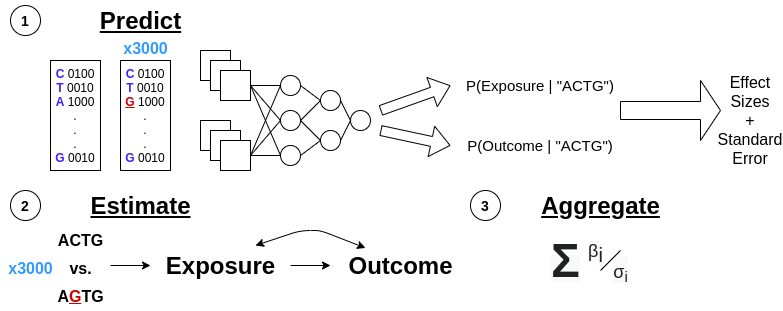
\includegraphics[width=.8\linewidth]{fig/model_overview.png}
    \vspace{-12pt}
    \caption{Graphical representation of Deep MR's high-level steps combining \textit{in silico} mutagenesis and MR (see Section \ref{sec:algo_overview}). \underline{Predict} corresponds to steps 1 through 4. \underline{Estimate} corresponds to step 5. \underline{Aggregate} corresponds to step 6}
    \vspace{-10pt}
    \label{fig:model_overview}
\end{figure*}

Saturation \emph{in silico} mutagenesis characterizes how a model's predictions for an input change as a result of all possible point mutations to the input. Saturation mutagenesis has been used to assess the learned representations of genomic deep learning models such as DeepBind \cite{alipanahi2015predicting}, cDeepBind \cite{gandhi2018cdeepbind}, DeepSEA \cite{zhou2015predicting}, and Basset \cite{kelley2016basset}. Here, we use saturation mutagenesis (combined with MC-dropout \cite{gal2016dropout}, see Section \ref{sec:dl_uncertainty}) to generate a set of estimated variant \textit{effect sizes} which we then provide as input to Mendelian randomization.

\subsection{Mendelian Randomization}

Mendelian randomization (MR) is a technique for estimating linear causal effects in the presence of potential unobserved confounders. MR is an instrumental variable method where the instrument(s) are genetic variants. While MR is typically used to estimate inter-phenotype causal effects from population-scale observational data (i.e., genome-wide association studies, GWAS), here we explore its application to estimating causal effects implied by model-generated data.


\subsubsection{Mendelian Randomization Assumptions}
MR only produces valid causal effect estimates under the following assumptions (Figure \ref{fig:model_overview} under \underline{Estimate}) \cite{lawlor2008mendelian}. Let $ Z $ be a variable we intend to use as an instrument (a genetic variant for example), $ X $ a purported cause (\textit{exposure}), and $ Y $ a purported effect (\textit{outcome}), and suppose that there may be unobserved confounding between $ X $ and $ Y $, denoted by $ U $. Then, MR gives an unbiased estimate of the causal effect of $X$ on $Y$ if:
\begin{compactenum}
    \item $ Z $ is independent of $ U $,
    \item $ Z $ is not independent of $ X $,  and
    \item $ Z $ only influences $ Y $ through $ X $.
\end{compactenum}

Recently developed MR methods such as Robust Adjusted Profile Score \cite{zhao2018statistical}, MR-Egger \cite{bowden2015mendelian}, and the modal-based estimator \cite{burgess2018modal} leverage multiple instruments to relax some of these assumptions without compromising the validity of results. In this work, we estimate causal effects using MR-Egger with the goal of being robust to invalid instruments.

\subsection{Uncertainty Estimates from Deep Learning Models}
\label{sec:dl_uncertainty}
For MR, we need standard error estimates for each predicted variant effect size. To acquire these, we use Monte Carlo Dropout (MC-dropout) \cite{gal2016dropout}. MC-dropout is motivated by showing that a typical deep learning model that uses dropout can be thought of as a variational approximation to Gaussian process regression/classification. In practice, MC-dropout involves enabling dropout at test time, making repeated predictions for each sequence (50 times in our case), and then computing the predictive mean and variance as described in \citet{gal2016dropout} (assuming classification). 

\section{Methods}
\begin{figure*}[ht]
\centering
\begin{subfigure}
\centering
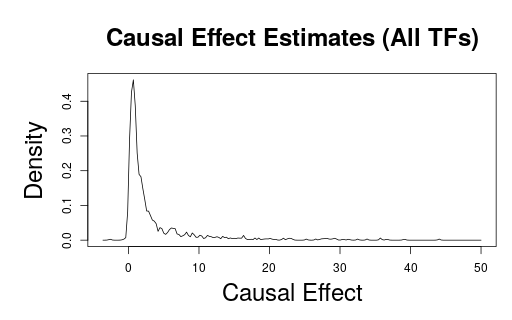
\includegraphics[width=.4\linewidth]{fig/all_tfs_ces_kde}
\end{subfigure}%
\vspace{-12pt}
\begin{subfigure}
\centering
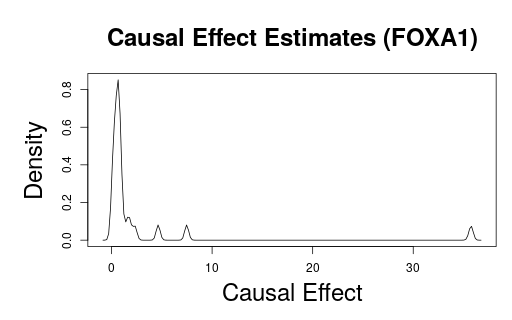
\includegraphics[width=.4\linewidth]{fig/HepG2_FOXA1_ces_kde}

\label{fig:sub2}
\end{subfigure}
\begin{subfigure}
\centering
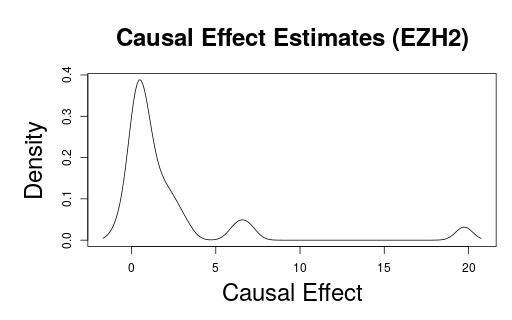
\includegraphics[width=.4\linewidth]{fig/HepG2_EZH2_ces_kde}
\end{subfigure}%
\vspace{-12pt}
\begin{subfigure}
\centering
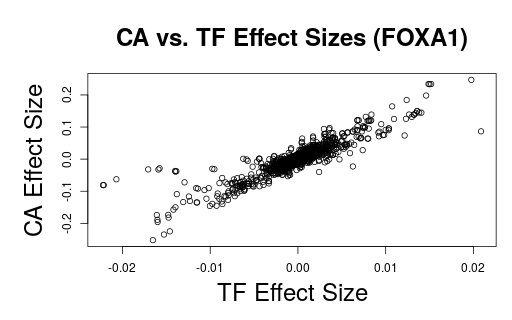
\includegraphics[width=.4\linewidth]{fig/HepG2_FOXA1_ex_eff_sizes_scatter.png}
\end{subfigure}%
\caption{Kernel density estimate of per-region causal effect estimates for all TFs (a) (top left), FOXA1 (b) (top right), and EZH2 (c) (bottom left). Example scatter plot showing the effect sizes for the median causal effect estimate sequence for FOXA1 (d) (bottom right).}
\label{fig:ces_kdes}
\vspace{-9pt}
\end{figure*}
\subsection{Method Overview}
\label{sec:algo_overview}
\begin{figure*}[htpb]
    \centering
    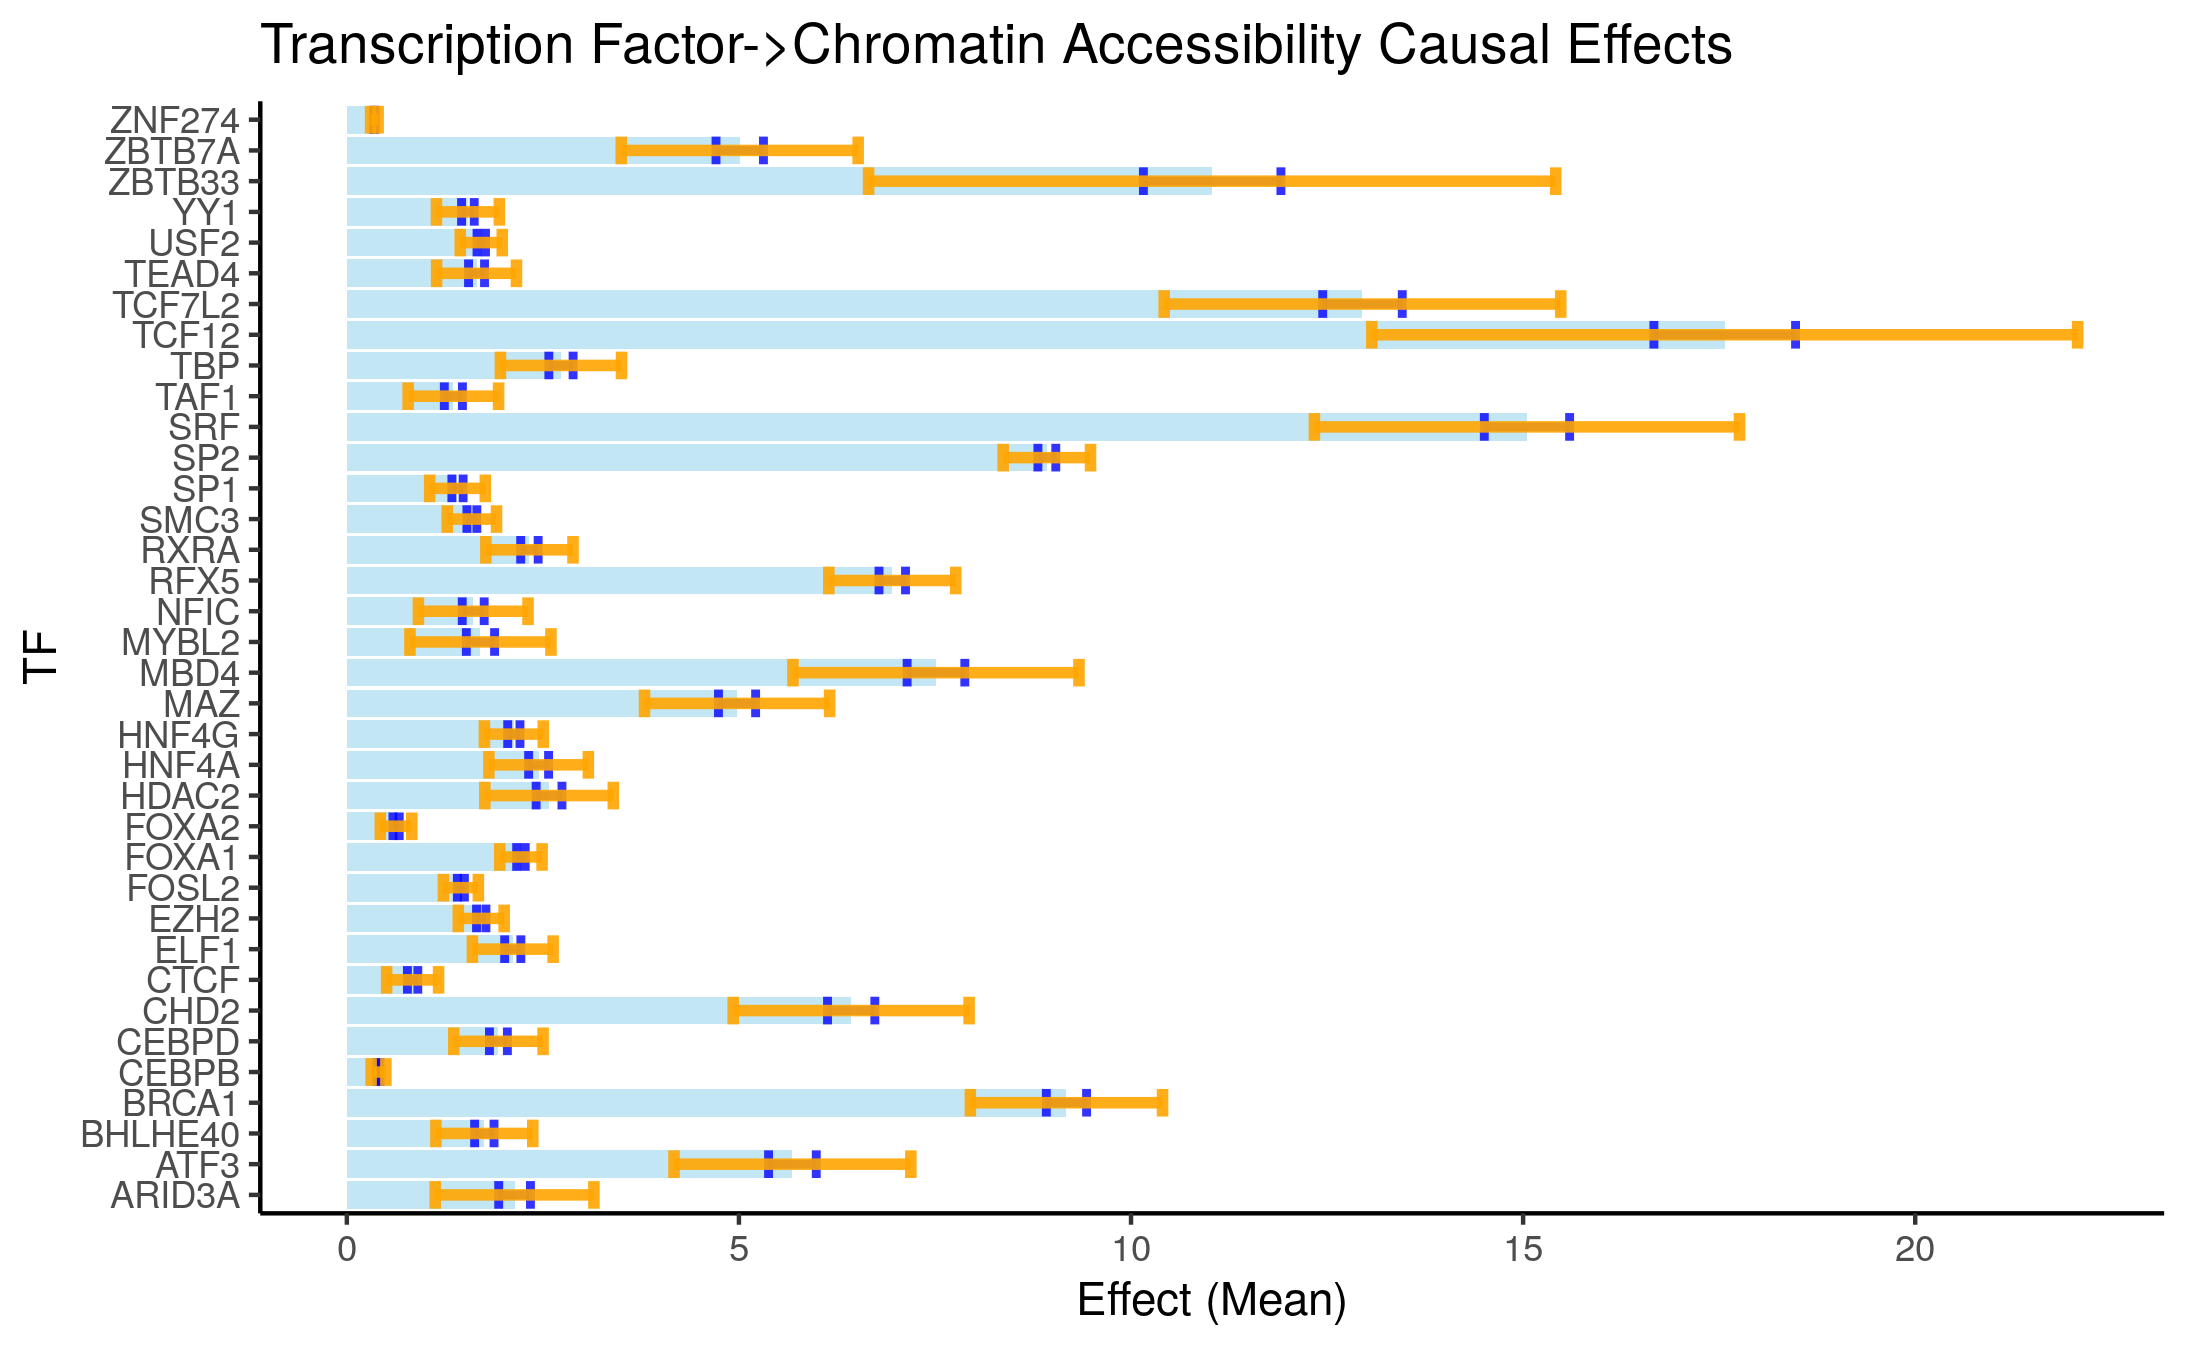
\includegraphics[width=14cm,height=9cm]{fig/overall_ces.png}
    \vspace{-12pt}
    \caption{Per-TF causal effect estimates output by Deep MR's final step. The light blue bars show the magnitude of the overall causal effect estimated by the meta-analysis. Orange bars show \( \tau \)'s magnitude and dark blue the standard deviation of the mean's.}
    \vspace{-10pt}
    \label{fig:overall_ces}
\end{figure*}

Deep MR estimates causal effect sizes between variables predicted by a multi-task model. It takes a trained model\footnote{The model could in principle be a regression or classification model, but we focus on classification in our experiments.} and a set of one-hot encoded sequences as input. In our case, the one-hot encoded sequence represents a sequence of nucleotides for the model to make predictions on.

Deep MR outputs local, sequence-specific causal effects and global, exposure-specific causal effects. It accomplishes this (see Figure~\ref{fig:model_overview} for a visual depiction) via the following steps for each exposure:
\begin{compactenum}
    \item Randomly sample sequences to predict exposure and outcome values for ``reference sequences''.
    \item Perform \textit{saturation in-silico mutagenesis} for each reference sequence to generate \( (\text{sequence\ length} \times \text{alphabet\ size} - 1) \) mutated sequences per reference sequence.
    \item For each reference and set of mutated sequences, use MC-dropout \cite{gal2016dropout} to generate predictive means and standard errors of binding probabilities for the reference and mutated sequences.
    \item Generate \( (\text{sequence length} \times \text{alphabet size} - 1) \) \textit{effect sizes} by subtracting each reference sequence's predictive mean from the corresponding mutated sequences' predictive means. Also, compute the standard errors of these differences.
    \item Estimate a per-exposure, per-sequence region causal effect by running MR on the effect sizes and their standard errors.
    \item Estimate overall per-exposure causal effects using a random effects meta-analysis.
\end{compactenum}


\subsection{Exposure and Outcome Effect Size \& Standard Error Estimation}

MR requires variant effect estimates for each mutation for both the exposure $X$ and outcome $Y$. Let $P(X=1 \mid Z, \theta) = f_X(Z,\theta)$ and $P(Y=1 \mid Z, \theta) = f_Y(Z,\theta)$ be the DL model for $X$ and $Y$ respectively with input sequence $Z$ and parameters $\theta$. Appealing to the interpretation of MC-dropout as approximate variational inference, the prediction for $X$ is $P(X=1 \mid Z) \approx \frac1N \sum_{n=1}^N f_X(Z, \theta^{(n)})$ where $n$ corresponds to different random dropout masks (analogously different draws from the variational posterior). Calculating this MC estimate for both the mutant sequence $m$ and reference $r$ we can obtain an unbiased estimate of the variant effect $\hat{\beta}_{ZX} = P(X=1 \mid Z=m) - P(X=1 \mid Z=r)$. We proceed analogously for the outcome $Y$.

A naive estimate of the standard errors (s.e.) would use $\text{var}[\hat{\beta}_{ZX}] = \text{var}{[P(X=1 \mid Z=m)]} + \text{var}{[P(X=1 \mid Z=r)]}$ with the variances estimated by MC. However, this would give inflated s.e.\ since it ignores statistical dependence resulting from $\theta$. We therefore instead use 
\begin{align*}
    \text{var}[\hat{\beta}_{ZX}] &= \text{var}{[P(X=1 \mid Z=m) - P(X=1 \mid Z=r)]} \\
    &= \frac1N \sum_{n=1}^N \left[f_X(m, \theta^{(n)}) - f_X(r, \theta^{(n)})\right]^2 - \hat{\beta}_{ZX}^2. 
\end{align*}
In practice this requires ensuring the dropout mask used for each mutated sequence is the same as for its corresponding reference sequence for each $n$. The s.e. for $\beta_{ZX}$ is then the square root of this expression. An analogous computation is performed to obtain the s.e. of $\beta_{ZY}$. 

% To estimate overall causal effects at the per-exposure level, we used an inverse-variance weighted random effects meta-analysis.


\section{Experimental Results}

To test Deep MR, we used a pre-trained DeepSEA~\cite{zhou2015predicting} model provided by the Kipoi library~\cite{avsec2019kipoi} to estimate the learned causal effects of 36 TFs on CA in the HepG2 cell type. For each TF we randomly sample 25 1000 base pair sequence regions (labelled as having binding of the TF) from DeepSEA's held-out test set\footnote{Full list found in supplementary Table 1 \hyperlink{https://www.nature.com/articles/nmeth.3547\#Sec12}{here}.}. This data was generated via processing the results of ChIP-seq (for TFs) and DNase-seq (for CA) experiments as part of the ENCODE project~\cite{encode2004encode}.

\paragraph*{Linear relationship between variant effects on TF binding and accessibility.}
We found TF and CA variant effect estimates were approximately linearly related across sequence regions and TFs (see e.g. effects for one sequence region for FOXA1 in Fig \ref{fig:ces_kdes}d). That we see a similar pattern for many sequences and TFs is suggestive that MR's linear effect assumption is valid in this setting.

\paragraph*{Causal effect estimates are mostly positive.}
All of the exposure-specific causal effect estimates are positive with \( \tau \) intervals that never include 0 (Figure~\ref{fig:overall_ces}). This defies our initial expectation that increased probability of binding of transcription repressors such as EZH2 would lower the probability of chromatin being accessible. Furthermore, the 25\% to 75\% quartile range for sequence-specific causal effect estimates is .64 to 3.54 (mode: 0.41, median: 1.36, see Figure~\ref{fig:ces_kdes}a's density plot for the whole distribution), and out of the 900 region-specific causal effect estimates, only 3 are negative. Together, these results suggest that increased binding of even repressive factors such as EZH2 locally increases CA (see Discussion).

\paragraph*{Sequence-specific causal effect variance.}
We inspected the sequence-level causal effect estimates for a known transcriptional activator, FOXA1, and transcriptional repressor, EZH2, in HepG2. The majority of causal effect estimates for both FOXA1 and EZH2 (Figures~\ref{fig:ces_kdes}b and~\ref{fig:ces_kdes}c respectively) are significantly non-zero but with absolute value \(<1\) (medians .70 and .75 respectively) with a few outliers greater than 5. Taken at face value, this implies that many sequence regions can be mutated in a way that impacts CA via effects on TF binding, some much more dramatically than others.

\paragraph*{Exposure-specific causal effect variance.}
The variance in exposure-specific causal effects (Figure~\ref{fig:overall_ces}) implies that the binding of certain TFs impacts accessibility throughout the genome much more than that of other TFs. An alternative hypothesis is that the varying impact on accessibility is specific to \emph{the sequences we sampled for each TF}. In future work we intend to distinguish these alternative explanations by more comprehensive sampling of bound sequence regions.

\section{Discussion}
In our experiment, Deep MR identified a consistent positive effect of TF binding on CA. Obtaining true causal effect estimates from MR requires relying on specific assumptions that we cannot guarantee hold here. Nonetheless, we believe this provides preliminary evidence that DeepSEA at least partially recovers meaningful relationships. We intend to follow up with work to:
\begin{compactitem}
    \item Verify Deep MR's sequence-level causal effect estimates by comparing to results from TF knockdown experiments.
    \item Apply Deep MR to outcomes other than accessibility that are more directly associated with active transcription (such as H3K27ac) to test whether negative causal effects are then detected for repressors.
    \item Investigate whether causal effect estimate heterogeneity comes from binding of co-factors/interaction effects with other TFs by estimating networks of TF interactions rather than just pairwise effects.
\end{compactitem}

\clearpage

\bibliography{deepmr}
\bibliographystyle{icml2020}
\end{document}


% This document was modified from the file originally made available by
% Pat Langley and Andrea Danyluk for ICML-2K. This version was created
% by Iain Murray in 2018, and modified by Alexandre Bouchard in
% 2019 and 2020. Previous contributors include Dan Roy, Lise Getoor and Tobias
% Scheffer, which was slightly modified from the 2010 version by
% Thorsten Joachims & Johannes Fuernkranz, slightly modified from the
% 2009 version by Kiri Wagstaff and Sam Roweis's 2008 version, which is
% slightly modified from Prasad Tadepalli's 2007 version which is a
% lightly changed version of the previous year's version by Andrew
% Moore, which was in turn edited from those of Kristian Kersting and
% Codrina Lauth. Alex Smola contributed to the algorithmic style files.
